\begin{savequote}[10cm] % this sets the width of the quote
\sffamily
``This is not Nam. This is bowling. There are rules!'' 
\qauthor{Walter Sobchak - The Big Lebowski}
\end{savequote}

\chapter{Another Chapter}
\graphicspath{{ch1/}} 


It's likely that you'll need another chapter, so here's a filler just to see
where it will go \cite{sample}. Also here is a figure \ref{lambda}, so
you can see how the \emph{hyperref} package works. Note the
hyperlinking of the citation and figure reference. This will only work if you have the \emph{foronline} option included for the MQThesis document class, at the top of thesis.tex.

\begin{figure}[tbp]  
\begin{center}
\setlength{\unitlength}{1cm}
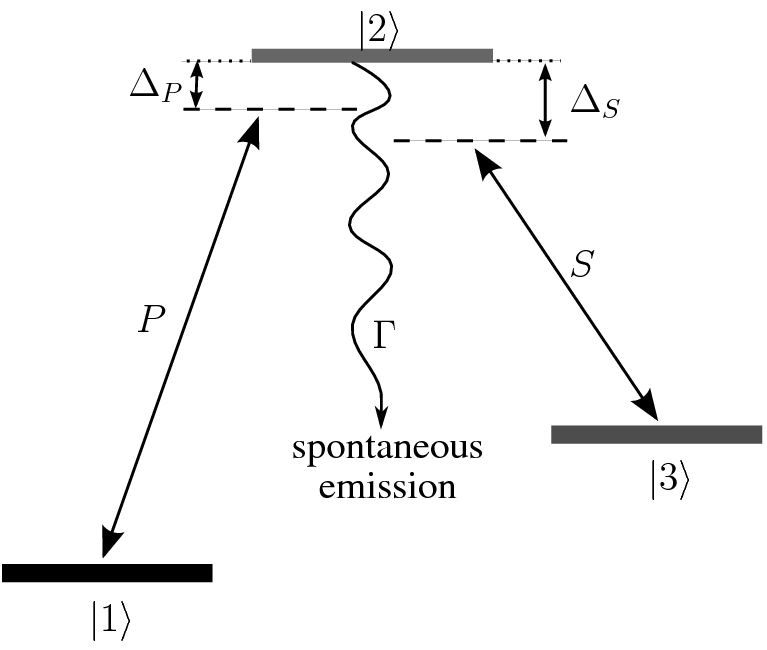
\includegraphics[width=8.4\unitlength]{lambda.png}
\end{center}
\caption{The $\Lambda$-type three-level energy scheme. States
$|1\rangle$ and $|2\rangle$ are coupled by the pump pulse $P$ which has a
detuning $\Delta_P$ from being exactly on resonance.  Similarly states
$|2\rangle$ and $|3\rangle$ are coupled by the Stokes pulse $S$ which has a
detuning $ \Delta_S$. State $|2\rangle$ is short lived with spontaneous emission
occurring out of the system}
\label{lambda}
\end{figure}

